\chapter{\label{sec:sampleprobefabrication}Sample probe fabrication}

\begin{figure}[h]
\centering
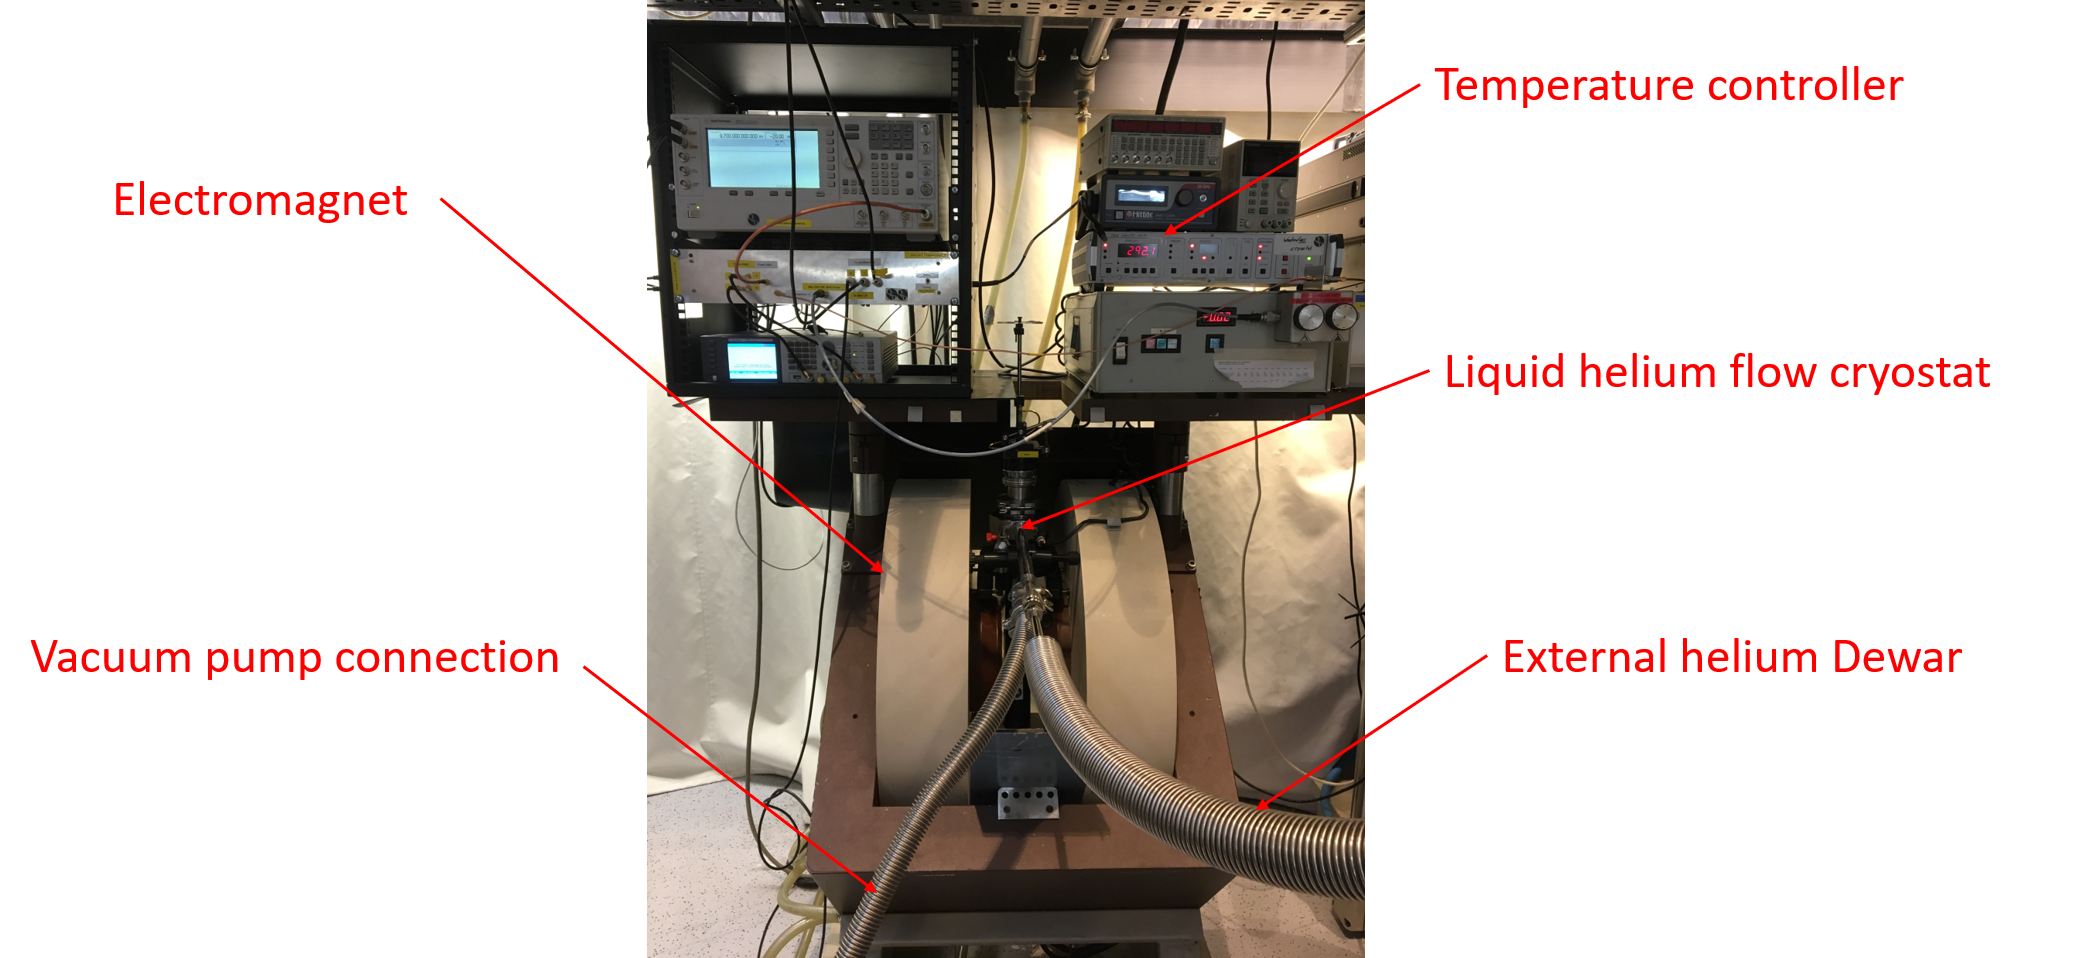
\includegraphics[height=0.32\textwidth,keepaspectratio]{cryostatimage}
\caption{\label{fig:experimentalsetup} Image of components of the EPR experimental set up.}
\end{figure}


\begin{figure}[H]
    \centering
    \begin{subfigure}[b]{0.4\textwidth}
        \centering
        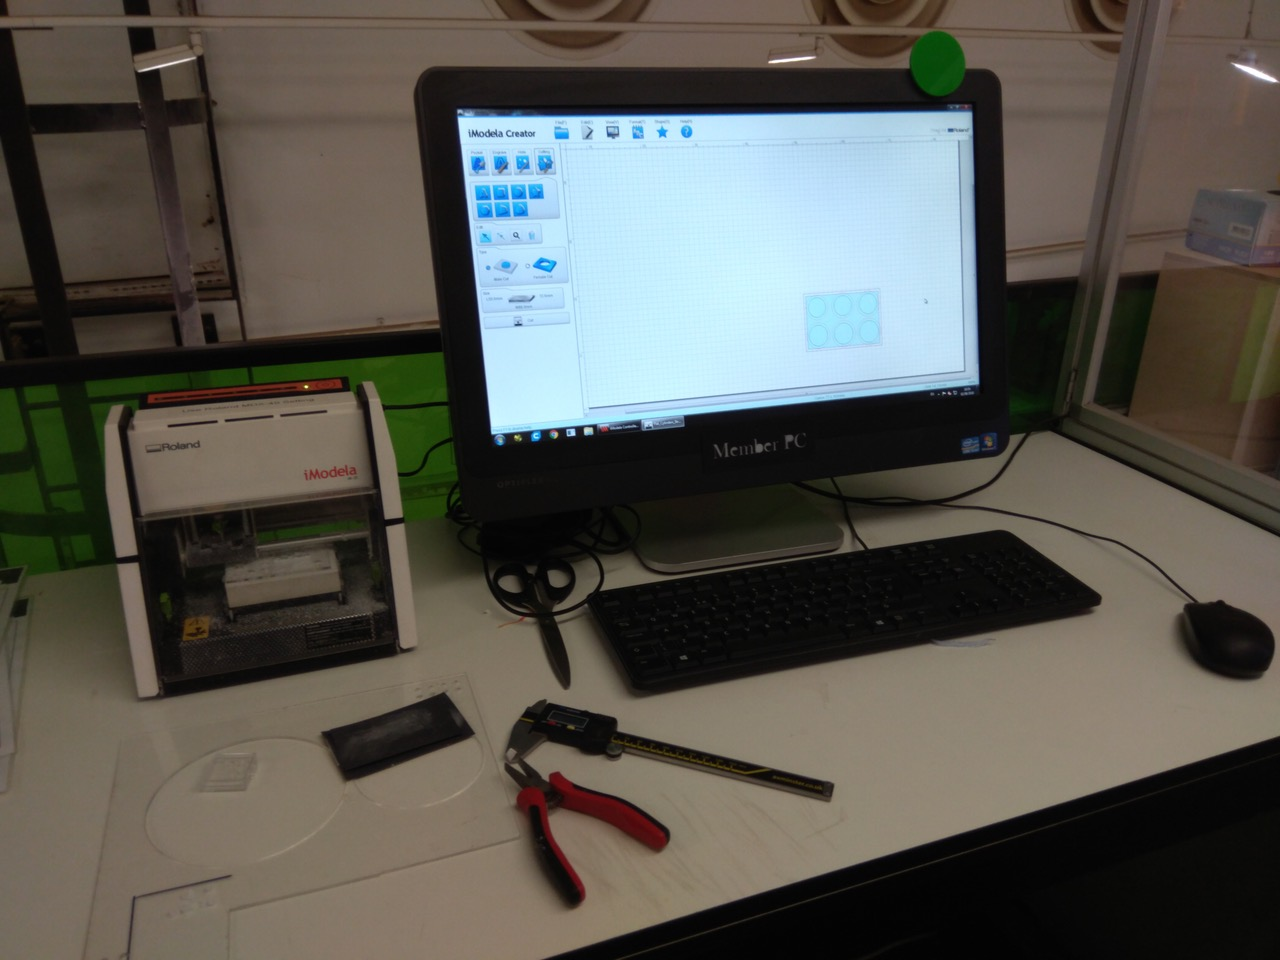
\includegraphics[width=\textwidth]{CNC3}
        \caption{}
    \end{subfigure}
%     \hfill
    \begin{subfigure}[b]{0.4\textwidth}
        \centering
        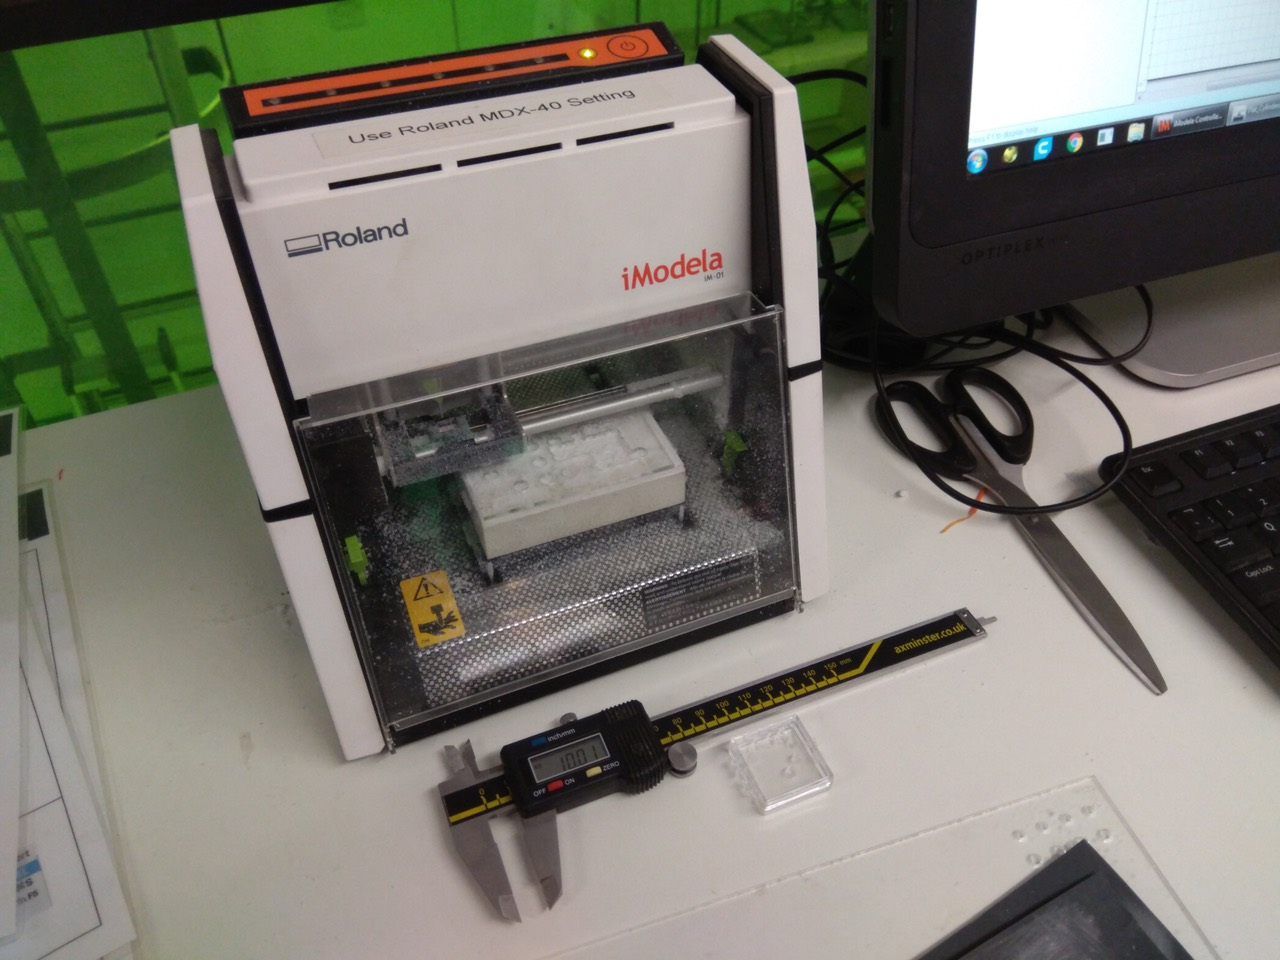
\includegraphics[width=\textwidth]{CNC1}
   \caption{}
   \end{subfigure}
       \begin{subfigure}[b]{0.4\textwidth}
        \centering
        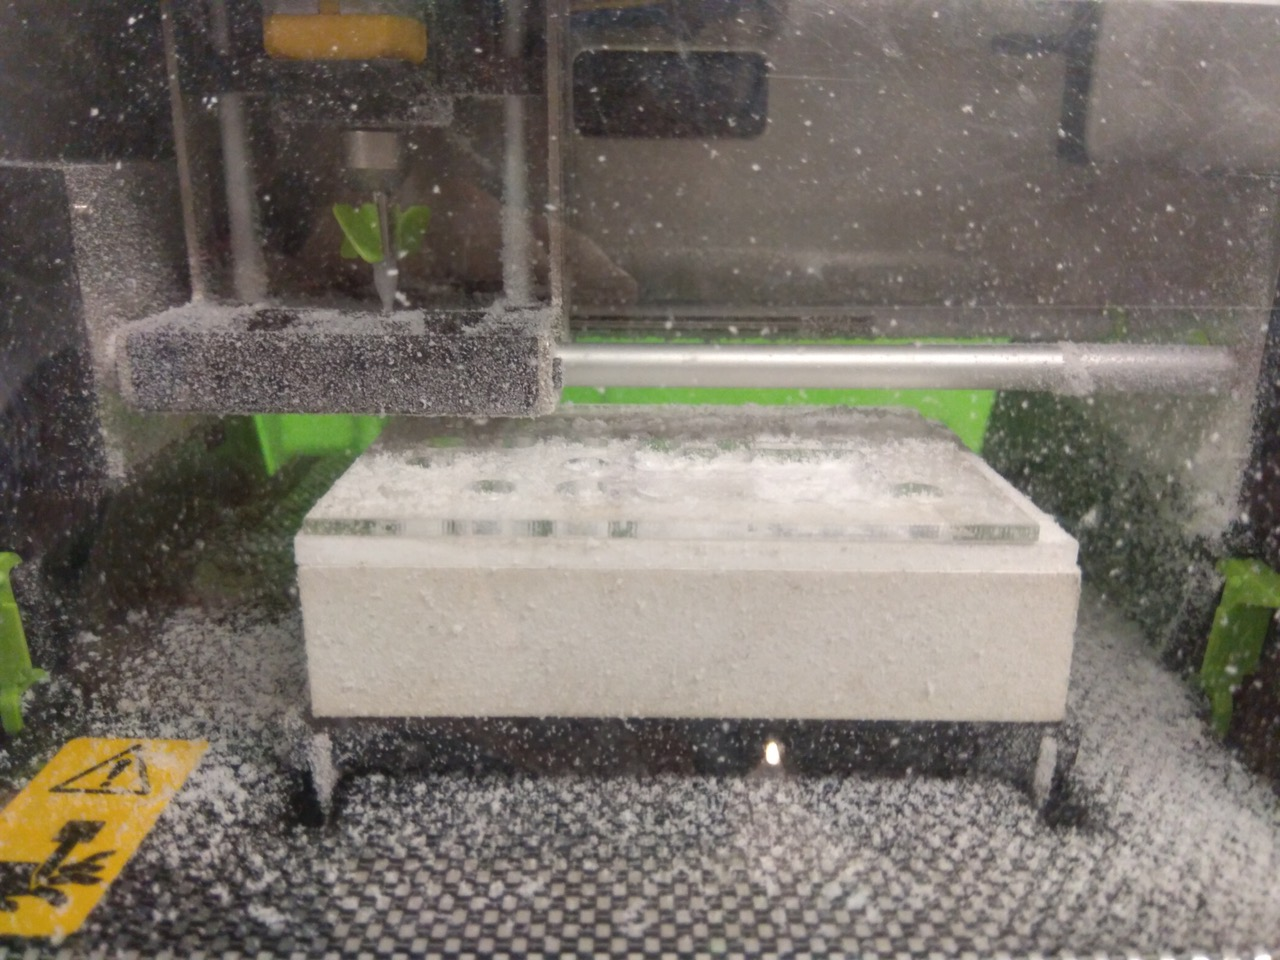
\includegraphics[width=\textwidth]{CNC2}
   \caption{}
   \end{subfigure}
   \caption{Images of the Computer numerical control (CNC) machine used to fabricate the acrylic sample holder pieces. (a) iModel creator software used to define the design. (b) CNC machine containing a drill piece which is used to mill the sample material. (c) Milling of cylindrical acrylic pieces.}
\end{figure}


\begin{figure}[H]
    \centering
    \begin{subfigure}[b]{0.35\textwidth}
        \centering
        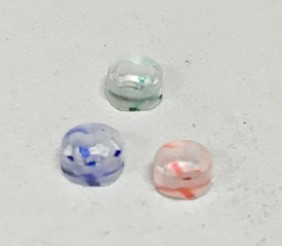
\includegraphics[width=\textwidth]{acrylicpieces}
        \caption{}
    \end{subfigure}
%     \hfill
    \begin{subfigure}[b]{0.3\textwidth}
        \centering
        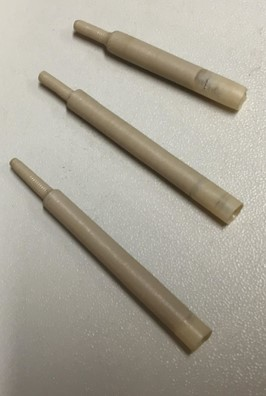
\includegraphics[width=\textwidth]{adapterrods}
   \caption{}
   \end{subfigure}
       \begin{subfigure}[b]{0.2\textwidth}
        \centering
        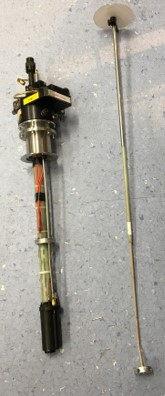
\includegraphics[width=\textwidth]{fullprobesetup}
   \caption{}
   \end{subfigure}
   \caption{Image of (a) the acrylic sample holders, (b) the adapter rods and (c) resonator probe (left) and rod pieces (right).}
\end{figure}


\begin{figure}[H]
    \centering
    \begin{subfigure}[b]{0.3\textwidth}
        \centering
        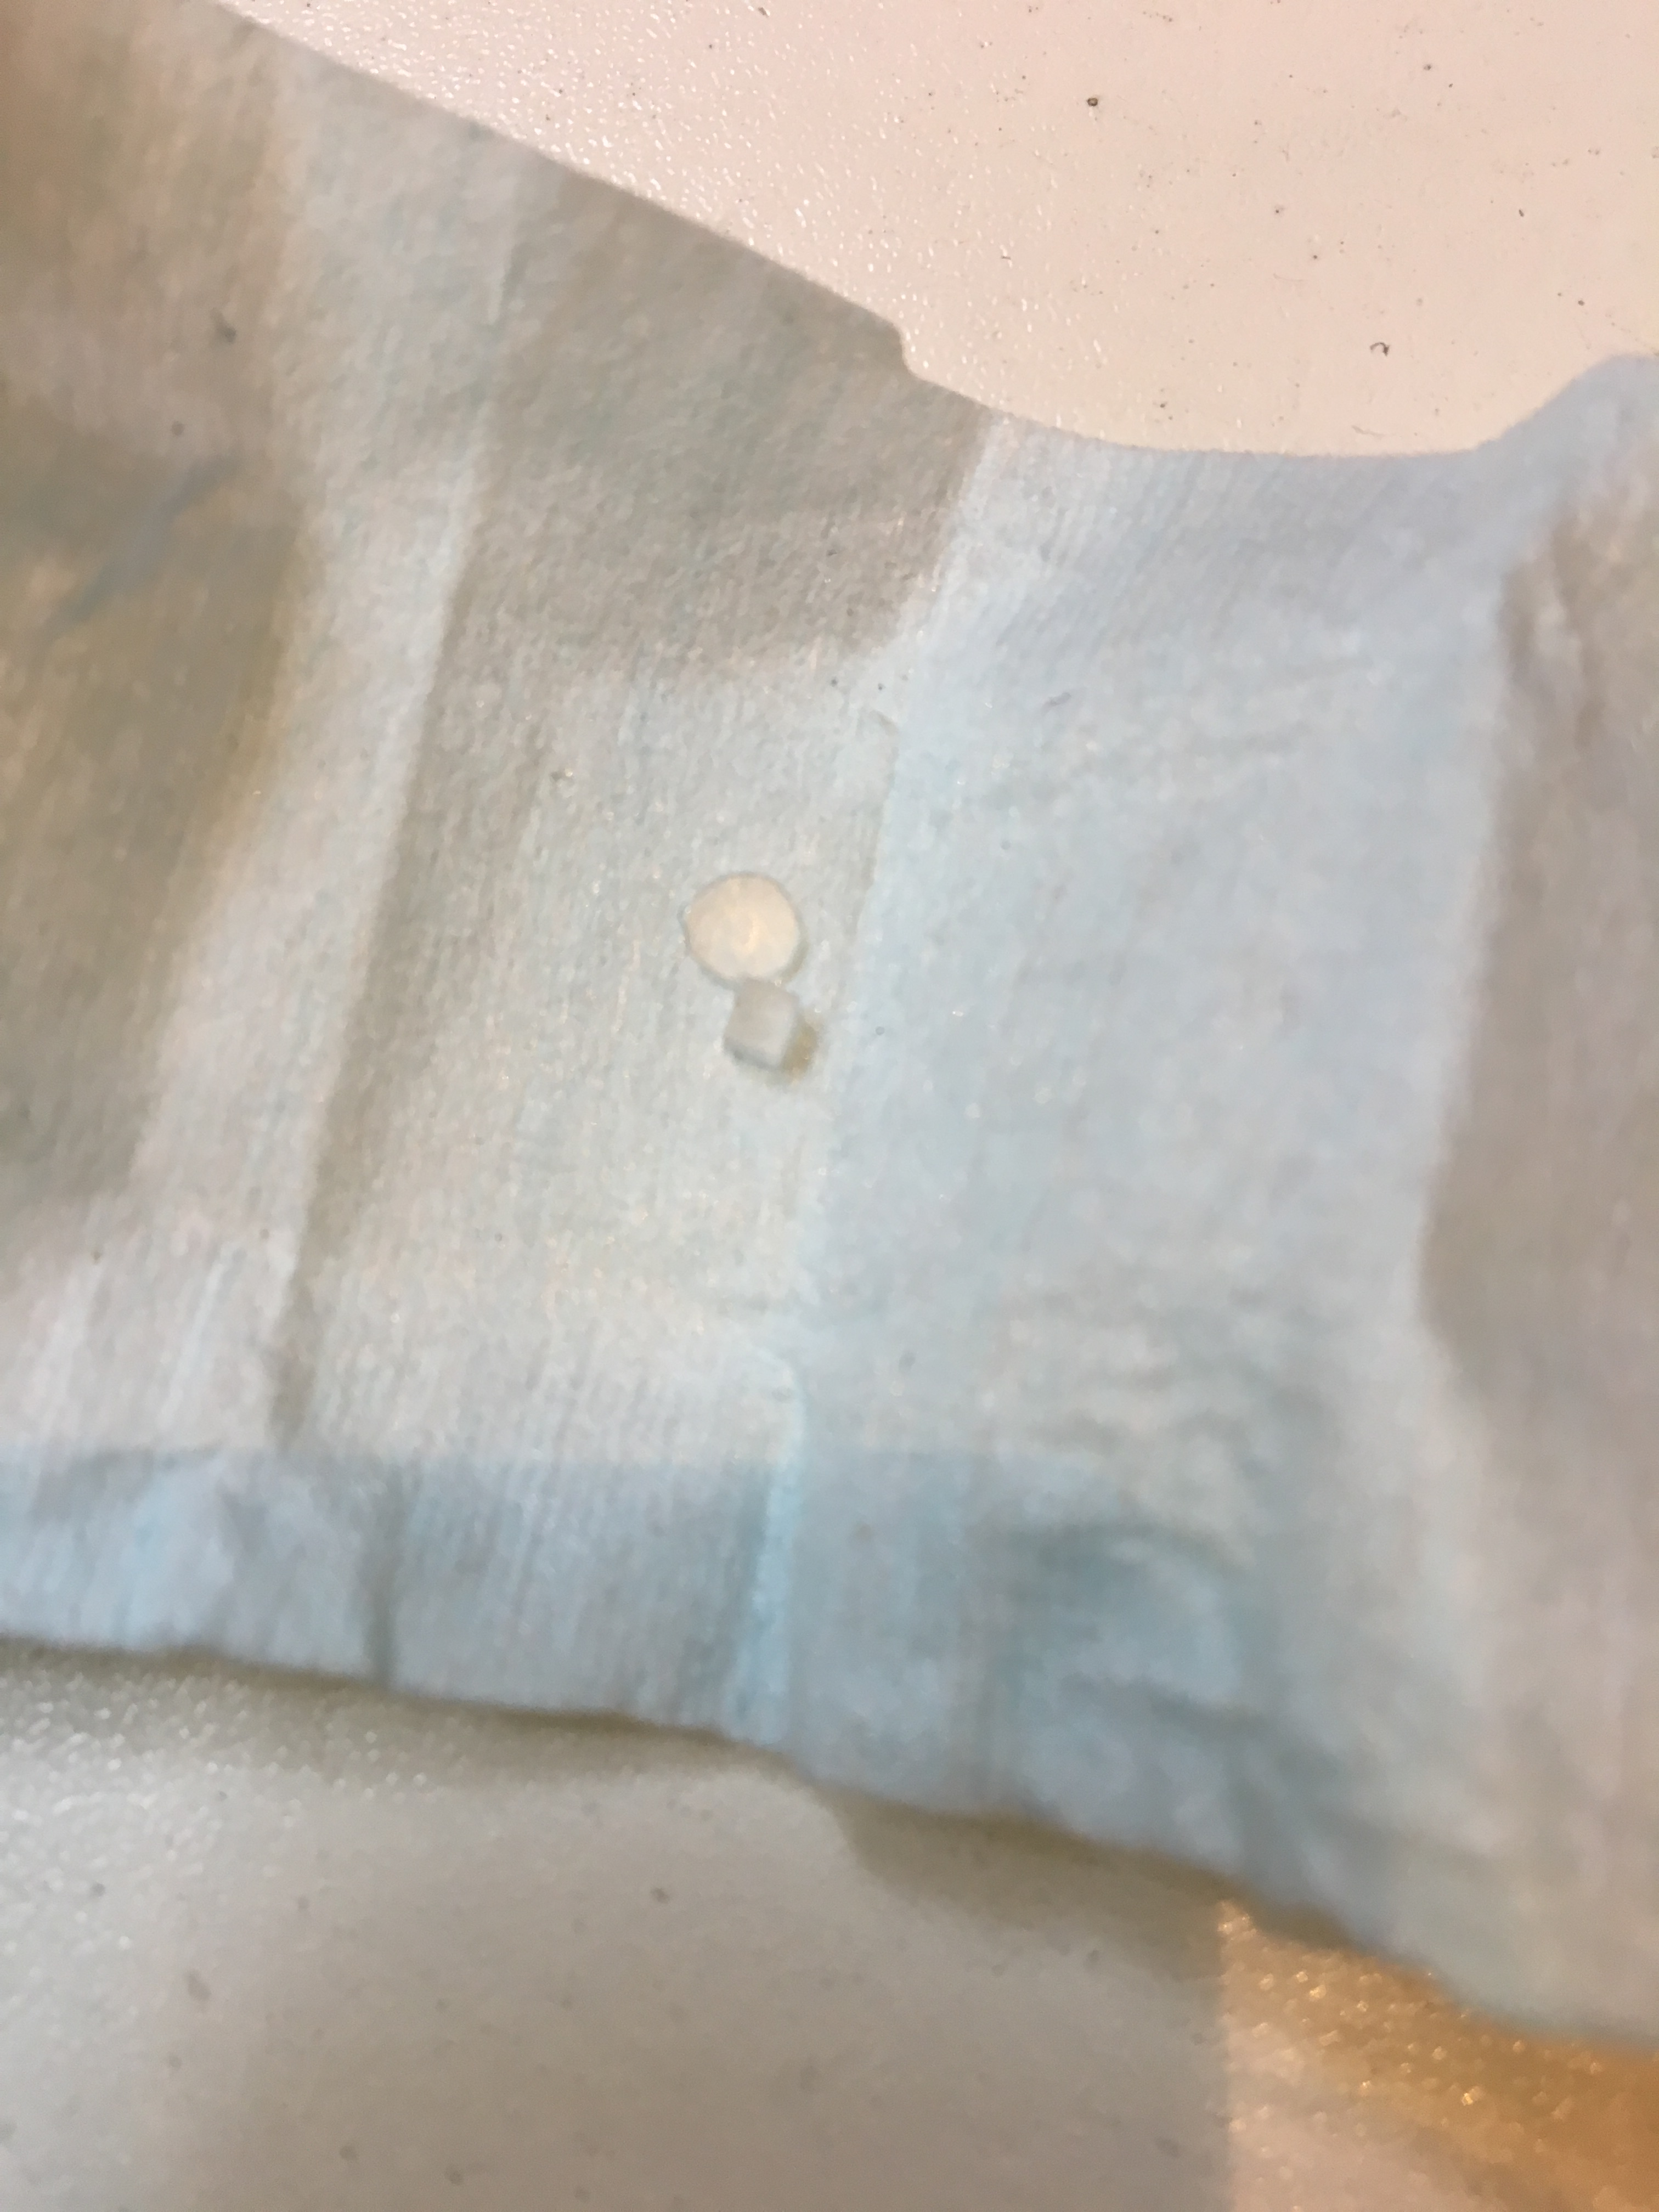
\includegraphics[width=\textwidth]{ybysosample}
        \caption{}
    \end{subfigure}
%     \hfill
    \begin{subfigure}[b]{0.3\textwidth}
        \centering
        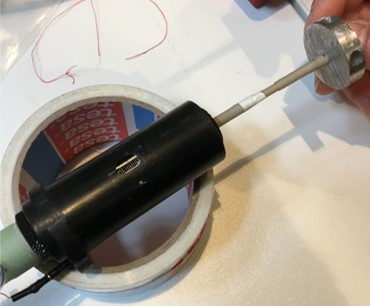
\includegraphics[width=\textwidth]{sampleloading}
   \caption{}
   \end{subfigure}
       \begin{subfigure}[b]{0.3\textwidth}
        \centering
        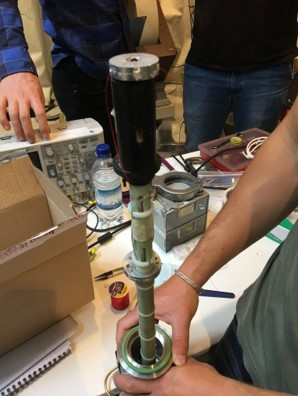
\includegraphics[width=\textwidth]{sampleloading2}
   \caption{}
   \end{subfigure}
   \caption{The transparent $^{171}$Yb$^{3+}$:YSO sample and circular acrylic piece used to separate the base piece from the sample when sample is inside the sample holder. (b) The cryogenic tape connecting the adapter to the base piece. (c) String connecting the base plate to the probe is used as a fail-safe.}
\end{figure}